\chapter{Simulação Distribuída de Eventos Discretos}

% Parágrafo 1: Revisar a déia inicial sobre o que é simulação, e dizer que a simulação é baseada em um modelo do problema

A simulação é uma técnica que permite prever e visualizar o comportamento de sistemas reais a partir de modelos matemáticos. As aplicações da simulação abrangem diversos benefícios, tais como: a possibilidade de antever possíveis problemas ou comportamentos indesejáveis de um sistema, auxílio na tomada de decisão sem a necessidade de intervir no sistema real, facilidade na manipulação e alteração dos modelos, economia de recursos (físicos e financeiros) durante a tomada de decisões, dentre outros.

% Parágrafo 2: Dizer que a simulação é um processo caro, e que é conveniente dividir entre vários computadores (distribuir a simulação)

Por demandar um intenso processamento computacional, a simulação por vezes pode se tornar uma opção demasiadamente custosa. Melhores algorítmos e métodos de simulação mais modernos são maneiras de tornar a simulação mais eficiente. Em paralelo à isto existe a possibilidade de se distribuir a simulação entre vários nós de um sistema, ou entre vários núcleos de uma máquina paralela. O uso desta técnica permite que certos processos sejam executados simultaneamente, acelerando assim a simulação.

% Parágrafo 3: Apresentar problemas como sincronização, comunicação, balanceamento de cargas, etc. devido à distribuição.

Em contrapartida, ao se dividir uma simulação entre vários nós em um sistema distribuído são criadas diversos novos requisitos ao sistema. Ítens como sincronização dos processos, comunicação entre os processos, balanceamento de cargas no sistema, entre outros devem ser gerenciados pela aplicação de simulação a fim de se garantir um resultado coerente do processo de simulação.


\section{Princípios da Simulação Baseada em Eventos Discretos}
% Parágrafo 4: Dividir o sistema em Processo lógicos e eventos discretos. Rever o conceito de timestamp de cada evento.

No paradigma da simulação discreta, três variáveis representam a simulação orientada a eventos:

\begin{itemize}
\item As variáveis internas do sistema;
\item Uma lista de eventos, denominada lista de eventos futuros. Esta lista abriga os eventos a serem executados;
\item Um relógio lógico global, que controla o processo de execução da simulação
\end{itemize}

Cada evento a ser executado possui uma marca  de tempo (\textit{timestamp}) que determina quando, no tempo lógico do sistema, este evento deve ser executado. O programa de simulação repetidamente retira o evento com o menor \textit{timestamp} da fila de eventos futuros para processa-lo.

Para a implementação da simulação distribuída, a estrutura da simulação tradicional, inerentemente sequencial, teve que sofrer adaptações para incorporar os conceitos de computação distribuída \cite{REED-MALONY}. Para isto, o sistema passou a ser dividido em processos lógicos que representam um processo de sistema real. Uma simulação é um conjunto com $n$ processos lógicos $p_{1}, p_{2}, p_{3}, ..., p_{n}$.

% Parágrafo 5: Dizer que cada processo lógico possui um relógio interno

Assim como o sistema de simulação possui um relógio lógico que representa o tempo lógico da simulação, ao se dividir a simulação em um sistema distribuído cada processo lógico possui um relógio lógico interno que representa o avanço do tempo de simulação para aquele processo lógico. Isso garante que os eventos a serem executados por um determinado processo lógico sejam executados no tempo lógico determinado pelo seu \textit{timestamp}. Portanto um processo lógico, se olhado isoladamente, possui as mesmas variáveis que um sistema de simulação sequencial: uma fila de eventos a serem executados, um relógio lógico interno e as suas variáveis internas.

% Parágrafo 6: Definir comunicação através de troca de mensagens

Porém em certos momentos um processo pode necessitar comunicar-se com outro processo lógico. Por exemplo, um processo pode enviar um evento para ser executado por outro processo lógico diferente. Esta comunicação é feita através de troca de mensagens. Um processo lógico deve ser capaz de enviar mensagens à outros processos lógicos que, por sua vez, devem ser capaz de receber estas mensagens. 

% Parágrafo 7: Definir o conceito de sincronização (timestamp das mensagens e LVT)

Assim como todo evento discreto, um evento enviado de um processo lógico à outro possui um \textit{timestamp} que indica quando este deve ser executado pelo processo lógico em questão. Porém, como os processos lógicos em um sistema distribuído não compartilham um mesmo relógio lógico (cada processo lógico possui seu próprio relógio interno), o sistema de simulação distribuída deve estar preparado para tratar situação de inconsistência da simulação.

Como cada processo lógico possui um relógio lógico interno independente, pode acontecer de um processo estar em um tempo lógico mais atrasado que os demais e enviar um evento para ser processado em um tempo que já foi superado pelo relógio lógico do processo que recebeu a mensagem. Assim como ilustrado na figura~\ref{fig:strag}, o processo em questão possui seu relógio lógico no tempo $t=24$ e recebe uma mensagem para ser processada no tempo $t=11$. Como o evento a ser processado possui um \textit{timestamp} menor que o relógio interno do processo lógico, o sistema encontra-se em um momento de inconsistência. Um sistema de simulação distribuída deve ser capaz de contornar tal situação.

\begin{figure}
  \centerline{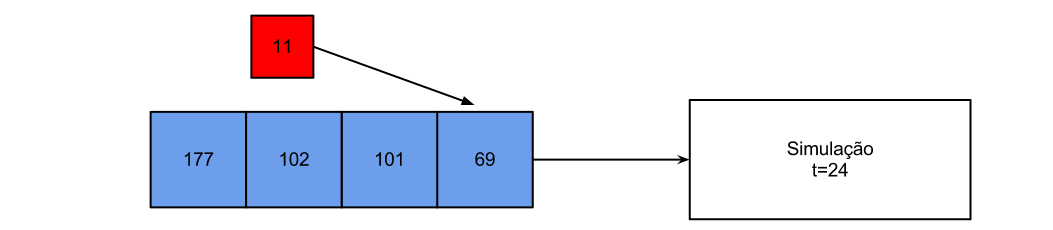
\includegraphics[scale=0.4]{straggler.png}}
  \caption{Mensagem \textit{straggler}.}
\label{fig:strag}
\end{figure}

\section{Categorias de protocolos de simulação}

% Parágrafo 1: breve discussão sobre as categorias de protocolos, explicando as principais diferenças

Para se garantir a sincronização dos processos lógicos na simulação distribuída são usados protocolos de sincronização, que garantem a consistência do sistema ao final da simulação. Os protocolos podem ser divididos em duas categorias quanto ao seu comportamento perante um inconsistência de causa e efeito no sistema: protocolos conservadores e protocolos otimistas. 

Um protocolo conservador evita que um erro de causa e efeito aconteça, garantindo que toda mensagem recebida por um processo lógico esteja dentro do tempo de execução daquele processo. Já um protocolo do tipo otimista não previne a ocorrência de inconsistências no sistema, mas provê mecanismos capazes de recuperar o sistema quando elas acontecem.

\subsection{Protocolos conservaticos}

Parágrafo 1: citar Srinivasan and Reynolds, explicando o conceito básico de um protocolo conservativo

Parágrafo 2: citar as implementacoes de [chandy e misra] e bryant, citando a necesidade de canais estaticos

Parágrafo 3: citar problema de bloqueio por esperar mensagem que contém um lvt inferior, citar também como contornar esse deadlock

Parágrafo 4: explicar porque é difícil resolver o problema de deadlock

Parágrafo 5: citar a desvantagem do conservativo por não aproveitar todo o paralelismo

Parágrafo 6: conclusão pessoal de porque não utilizar o protocolos conservativos

\subsection{Protocolos Otimistas}

Parágrafo 1: explicação inicial do conceito de protocolo otimista e citar o conceito de rollback

Parágrafo 2: Citar o time warp, contextualizando como foi desenvolvido, em qual época e por quem

Parágrafo 4: Citar o Rollback Solidário como alternativa ao Time Warp

\section{O protocolo \textit{Time Warp}}

Parágrafo 1: Explica por que o Time Warp é otimista, citando o fato de nao impedir a ocorrência de erros de causa e efeito

Parágrafo 2: Citar como um erro de causa e efeito pode acontecer, e o que deve ser feito quando isso acontece: o rollback

Parágrafo 4: Citar implementações do protocolo

Parágrafo 5: Explicar o comportamento individual de um processo lógico (tirar o eventos com menor timestamp da lista de eventos futuros, etc.)

\subsection{Detecção e Tratamento de Inconsistências}

Parágrafo 1: Mostrar que o sistema pode receber mensagens que causam erro de causa e efeito.

Parágrafo 2: Explicar o comportamento ao receber uma mensagem straggler.

Parágrafo 3: definir a diferença entre rollback primário e rollback secundário

\subsection{Anti-Mensagens}

Parágrafo 1: Explicar o que é uma antimensagem

Parágrafo 2: mostrar que antimensagens podem se referir a um evento já processado, ou a um evento que ainda esta na fila de eventos futuros

Parágrafo 3: Tratar o caso da antimensagem chegar antes da mensagem

\subsection{Considerações Finais}


\section{O protocolo \textit{Rollback} Solidário}

Parágrafo 1: Apresentar a principal diferença do rollback solidário

Parágrafo 2: explicar que, em caso de erro de causa e efeito, todos os processos executam rollback em conjunto

Parágrafo 3: introduzir o conceito de checkpoint, checkpoint global e checkpoint local.

\subsection{Comportamento Geral do Protocolo Rollback solidário}

Trazer uma idéia básica do Rollback solidário em linhas gerais

\subsection{Estados Locais e Estados Globais}

Parágrafo 1: Definição de um estado local como sendo os valores das variáveis do processo em questão em um determinado tempo

Parágrafo 2: Definição de estado global como sendo um conjunto de estdaos de cada processo.

\subsection{Cortes Globais Consistentes}

Parágrafo 1: Apresentar o conceito de precedência causal

Parágrafo 2: Definir corte 

Parágrafo 3: definir corte consistente utilizando precedência causal

\subsection{Relógios Lógicos e Relógios Vetoriais}

Parágrafo 1: Apresentar o conceito de relógio lógico

Parágrafo 2: Mostrar que o relógio lógico não representa a precedência causal em um sistema distribuído

Parágrafo 3: Apresentar o conceito de relógio vetorial

\subsection{Checkpoints Globais Consistentes}

Parágrafo 1: Definir o que é um checkpoint: um ponto de retorno que foi, de alguma forma, armazenado de forma persistente

Parágrafo 2: a necessidade de se garantir que um checkpoint seja consistente

Parágrafo 3: associação de checkpoint consistente com corte consistente

\subsection{Obtenção de Checkpoint Semi-Síncrono}

Parágrafo: introduzir o processo observador

Parágrafo: Introduzir o vetor de dependência

Parágrafo: Mostrar como a troca de mensagem deve levar o vetor de dependências, e como este deve ser atualizado no processo que recebeu a mensagem

Parágrafo: mostrar como o processo observador monta uma linha de recuperação através da matriz de dependências

Parágrafo: demonstrar que um checkpoint global consistente é formado por checkpoints locais que não possuem relação causal entre si


\subsection{Tratamento dos Rollbacks na Abordagem Semi-Síncrona}

Parágrafo: Explicar o comportamento de um processo ao receber uma mensagem straggler 

Parágrafo: Falar sobre a atuação do processo observador (escolher a linha de retorno, avisar o rollback à todos em broadcast, etc.)

Parágrafo: Falar sobre o reinício da simulação após o Rollback

\subsection{Considerações Finais}


\section{Balanceamento de cargas}

Parágrafo: apresentar o balanceamento de carga como fator determinante no desempenho de uma simulação distribuída

Parágrafo: Introduzir o conceito de escalonamento de processos como meio de prover o balanceamento de cargas

Parágrafo: por fim mostrar que para prover o balanceamento de cargas temos que possibilitar que um processo lógico migre de um nó do sistema para outro

\subsection{O Uso de Agentes Móveis Para Prover Mobilidade}

Parágrafo: O que é um agente móvel

Parágrafo: Falar sobre a implementação feita por Antonio, Walbon e Takahashi - 2010

Parágrafo: Outras implementações feitas usando agentes móveis

\subsection{Requisitos Para Mobilidade de um Processo Lógico}

Parágrafo: explicar quais as funcionalidades de agentes móveis que precisamos (migração)

Parágrafo: Abstrair o conceito de ambiente e processo lógico: um ambiente abriga diversos processos lógicos

Parágrafo: Mostrar a idéia de migrar um processo de um ambiente para outro, a fim de prover o balanceamento

\subsection{Considerações Finais}
